\documentclass[twoside]{article}

\usepackage[sc]{mathpazo} 
\usepackage[spanish, es-tabla]{babel}
\usepackage[utf8]{inputenc}

\usepackage[hmarginratio=1:1,top=32mm,columnsep=20pt]{geometry} % Document margins
\usepackage{multicol} % Used for the two-column layout of the document
\usepackage[hang, small,labelfont=bf,up,textfont=it,up]{caption} % Custom captions under/above floats in tables or figures
\usepackage{mathtools}
\usepackage{float} % Required for tables and figures in the multi-column environment - [H] needed
\usepackage{hyperref} % For hyperlinks in the PDF with labels

\usepackage{abstract} % Allows abstract customization
\renewcommand{\abstractnamefont}{\normalfont\bfseries} % Set the "Abstract" text to bold
\renewcommand{\abstracttextfont}{\normalfont\small\itshape} % Set the abstract itself to small italic text

\usepackage{titlesec} % Allows customization of titles

\titleformat{\section}[block]{\large\scshape\centering}{\thesection.}{1em}{} % Change the look of the section titles
\titleformat{\subsection}[block]{\large\centering}{\thesubsection.}{1em}{} % Change the look of the section titles

\usepackage{fancyhdr} % Headers and footers
\pagestyle{fancy} % All pages have headers and footers
\fancyhead{} % Blank out the default header
\fancyfoot{} % Blank out the default footer
\fancyhead[C]{Speckle% based on TRACS 
\hspace{4pt} $\bullet$ \hspace{4pt} Diciembre 2018 } % Custom header text
\fancyfoot[RO,LE]{\thepage} % Custom footer text

%----------------------------------------------------------------------------
%	   TITLE SECTION
%----------------------------------------------------------------------------

\title{
	\vspace{-15mm}
	\fontsize{28pt}{10pt}
	\selectfont\textbf{Estudio y Simulación del Efecto de Speckle}% Article title
}

\author{
	\large
	\textsc{Jaime D\'iez Gonz\'alez-Pardo}\\[4mm]
	\fontsize{28pt}{10pt} Universidad de Cantabria \\ % Your institution
	%\thanks{A thank you or further information}\\[2mm] % Your name
	\normalsize Fotónica \\ 
	%\normalsize{Compañeros:} \textsc{NOMBRE COMPANEROS }\\%\normalsize \href{mailto:john@smith.com}{john@smith.com} % Your email address
	%\vspace{5mm}
}

\date{ \today }


%----------------------------------------------------------------------------
%      · DOCUMENT
%----------------------------------------------------------------------------

\begin{document}


	\maketitle % Insert title


	\thispagestyle{fancy} % All pages have headers and footers

%----------------------------------------------------------------------------
%	  ABSTRACT
%----------------------------------------------------------------------------

	\begin{abstract}

		\noindent% Dummy abstract text

			Se ha simulado un espejo formado por pequeños espejos más pequeños con forma hexagonal y diferente fase cada uno, para tratar de estudiar el fenómeno de Speckle. En una primera parte se han simulado tres espejos diferentes: uno formado por un único espejo sin fase, otro formado por pupilas del tamaño del espejo grande, y otro en el que las pupilas eran más pequeñas que el espejo grande. Para los dos  primeros casos se ha obtenido la mancha de Airy, con algunas diferencia. Sin embargo en el tercer caso se ha obtenido un patrón de Speckle. Por último se ha tratado de recomponer una imagen a la que se le ha aplicado diferencias aleatorias en su fase a partir del fenómeno de Speckle.

	\end{abstract}

%----------------------------------------------------------------------------
%	  ARTICLE CONTENTS
%----------------------------------------------------------------------------

	\begin{multicols}{2} % Two-column layout throughout the main article text

		\section{Introducción} % Scope of the project = rad effects + minimization
							 
			El estudio de la interferometría Speckle consiste en el análisis del patrón de intensidades producidas por diferentes frentes de onda coherentes pero con diferencisas de fases.

			El caso más claro de este fenómeno se encuentra a la hora de tratar de observar las estrellas. Los frentes de onda esféricos emitidos por la estrella y que llegan a la Tierra en forma de frentes de onda planos de igual fase, debido a la gran distancia de la Tierra a la estrella, sufre un cambio de fase diferente en cada uno de sus puntos debido al efecto de la atmósfera en el frente de onda. Esto produce que al tratar de observar la imagen de la estrella, se obtenga el patrón propio al Speckle. 

			Una de las formas de corregir dicho efecto es mediante la utilización de pequeños espejosque forman una lente mayor para capturar la imagen, a los cuales se les induce una determinada inclinación que altera la fase del frente de onda corrigiendo el patrón.

				\begin{figure}[H]
					\centering
					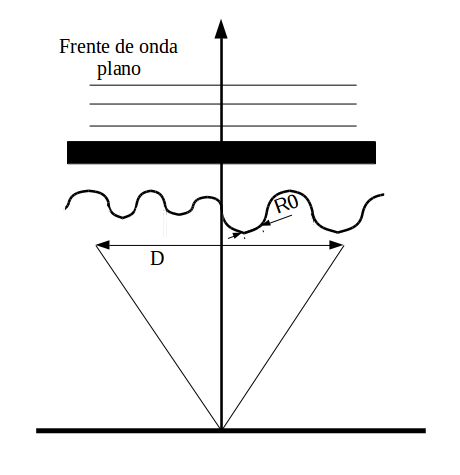
\includegraphics[scale=0.25]{Esquema.png}
					\caption{\label{Img:Esquema}Esquema del sistema simulado para estudiar el efecto Speckle. En la imagen $D$ corresponde al tamaño de la lente o Espejo del telescopi y $R0$ a la aproximación del frente de onda aleatorio en la cuál el frente de onda es constante y se puede aplicar la corrección.}
				\end{figure}

			Para el caso de un foco puntual, si no hubiese cambios en la fase se debería obtener la mancha de Airy. Para el efecto de Speckle se pueden obtener también diferentes aproximaciones a este patrón en función de $D$ y $r_0$:

				\begin{equation}
					\begin{matrix}
						D/r_0 >> 1 & \rightarrow & Imagen \neq Airy
						\\
						D/r_0 << 1 & \rightarrow & Imagen=Airy
					\end{matrix}
					\label{eq:airy}
				\end{equation}

		\section{Desarrollo Experimental}

			El estudio del efecto Speckle producido por diferencias en la fase del frente de onda se ha realizado mediante una simulación a partir del código \cite{Speckle} escrito por el alumno en el lenguaje Python.

			Para crear cada uno de los espejos o pupilas se ha utilizado una clase llamada Espejo que crea los espejos teniendo en cuenta el tamaño del campo, el tamaño del espejo o pupila, forma del espejo e inclinación. La forma utilizada para las puilas pequeñas ha sido la de un hexágono, ya que ésta te permite poder cubrir todo el espacio sin dejar huecos, la forma del espejo grande ha sido circular. En el apéndice \ref{appen:Espejo} se muestra como se ha obtenido la matriz para el espejo grande. El resultado de la simulación obtenido corresponde al rebote de la imagen en el espejo, que equivalente a la transformada de Fourier.

			En el caso del espejo formado por pupilas más pequeñas, se ha creado una matriz del tamaño del campo a estudiar relleno de las upilas pequeñas de tal manera que cubran toda la matriz, y se ha multiplicado dicha matriz por la del espejo grande compuesta de 0 y 1.

			La simulación se ha dividido en dos partes: En la primera parte se ha realizado el estudio considerando una fuente puntual utilizando tres espejos diferentes y en la segunda parte se ha tratado de corregir una imagen, a la que se le han aplicado cambios en la fase de forma aleatoria, aplicando la fase contraria en un espejo formado por pupilas pequeñas y recuperando dicha imagen.

			En la primera parte el primer espejo utilizado ha consistido en un único espejo circular sin fase, el segundo espejo utilizado se ha realizado utilizando pupilas del tamaño del espejo grande pero con forma hexagonal y con fase; y el último espejo utilizado ha consistido de varias pupilas hexagonales más pequeñas que el espejo grande y con fase aleatoria.

		\section{Resultados}

			Durante toda la simulación se ha utilizado un campo (tamaño de la matriz) cuadrado de $512\times512$

			\subsection{Fuente Puntual}

				Para esta primera parte se ha utilizado un tamaño de espejo grande de diámetro $D = 64$.

				La primera simulación realizada ha sido sin incluir pupilas más pequeñas ni ningún tipo de fase. En la Figura \ref{Img:airy-normal} se muestran imágenes del espejo utilizado (gráfica de la izquierda) y del campo obtenido (gráfica de la derecha).

					\begin{figure}[H]
						\centering
						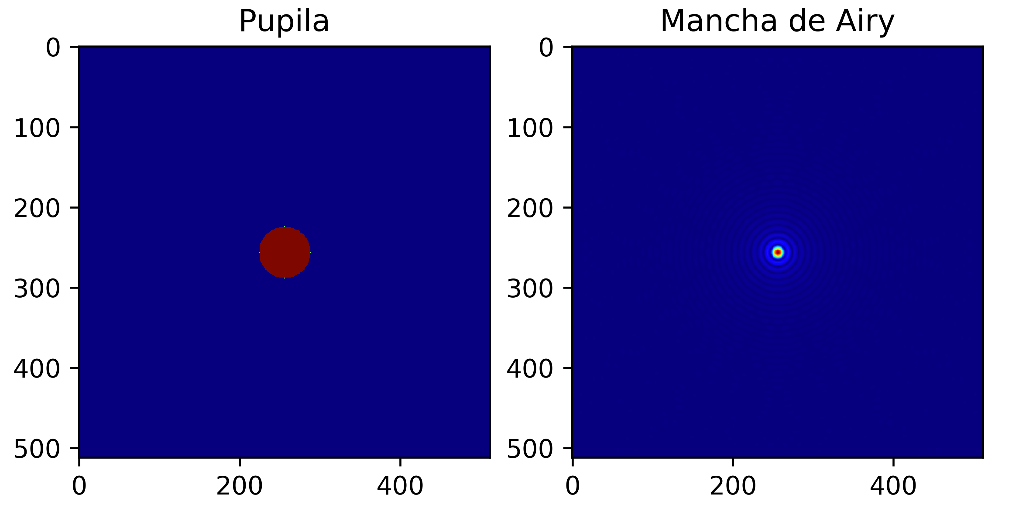
\includegraphics[scale=0.2]{Airy.png}
						\caption{\label{Img:airy-normal}Espejo utilizado sin pupilas ni fase (gráfica de la izquierda) y del campo obtenido (gráfica de la derecha).}
					\end{figure}

				En la segunda simulación realizada se han introducido pupilas con una cierta fase aleatoria con forma de hexágono para formar el espejo grande, en este caso el tamaño de las pupilas es el mismo que el del espejo grande $r_0 = D = 64$.

				En la Figura \ref{Img:airy-fase} se muestran imágenes del espejo utilizado (gráfica de la izquierda) y del campo obtenido (gráfica de la derecha).

					\begin{figure}[H]
						\centering
						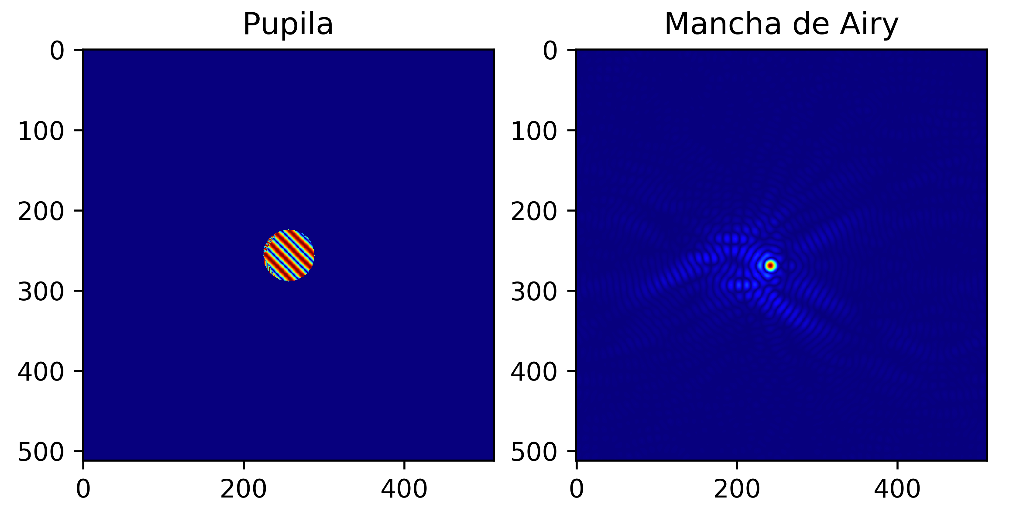
\includegraphics[scale=0.2]{Airy_Fase.png}
						\caption{\label{Img:airy-fase}Espejo utilizado con pupilas con fase de tamaño $r_0 = D = 64$ (gráfica de la izquierda) y del campo obtenido (gráfica de la derecha).}
					\end{figure}

				Por último, se han utilizado varias pupilas de tamaño menor a $D$ para formar el espejo, en este caso se han utilizado pupilas de tamaño $r_0 = 8$ y fase aleatroia para cada una de ellas.

				En la Figura \ref{Img:speckle} se muestran imágenes del espejo utilizado (gráfica de la izquierda) y del campo obtenido (gráfica de la derecha).

				\begin{figure}[H]
					\centering
					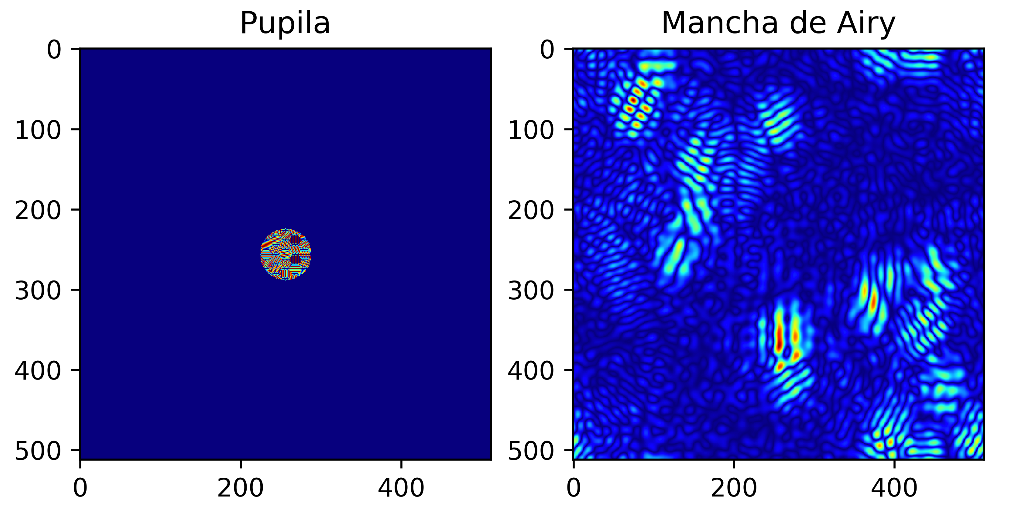
\includegraphics[scale=0.2]{SpeckleTotal.png}
					\caption{\label{Img:speckle}Espejo utilizado con pupilas con fase de tamaño $r_0 = 8$ (gráfica de la izquierda) y del campo obtenido (gráfica de la derecha).}
				\end{figure}

			\subsection{Imagen Fuente}

				Por último, se ha tratado de simular la corrección de speckle de una imagen a la que se le ha modificado de forma aleatoria la fase en cada punto. Para poder obtener la imagen real se ha aplicado la transformada de Fourier dos veces.

				Para poder observar la diferencias al aplicar la corrección de speckle o no se han realizado las simulaciones dos veces, la primera con un espejo sin pupilas ni fase (coma la utilizada en la imagen \ref{Img:airy-normal}) y otra con pupilas más pequeñas y con fase contraria a la de la imagen fuente (como la utilizada en la imagen \ref{Img:speckle}).

				Para esta parte el tamaño del espejo grande utilizado es de $D = 256$ y, para el caso del espejo con pupilas, el tamaño de las pupilas de $r_0 = 16$.

				En la Figura \ref{Img:nasa} se muestran las gráficas obtenidas. La primera columna corresponde a la imagen fuente, la segunda columna al espejo utilizado y la columna de la derecha a la imagen obtenida. La fila de arriba es sin aplicar la corrección de speckle y la de abajo con la corrección. 

				\end{multicols}
					\begin{figure}[H]
						\centering
						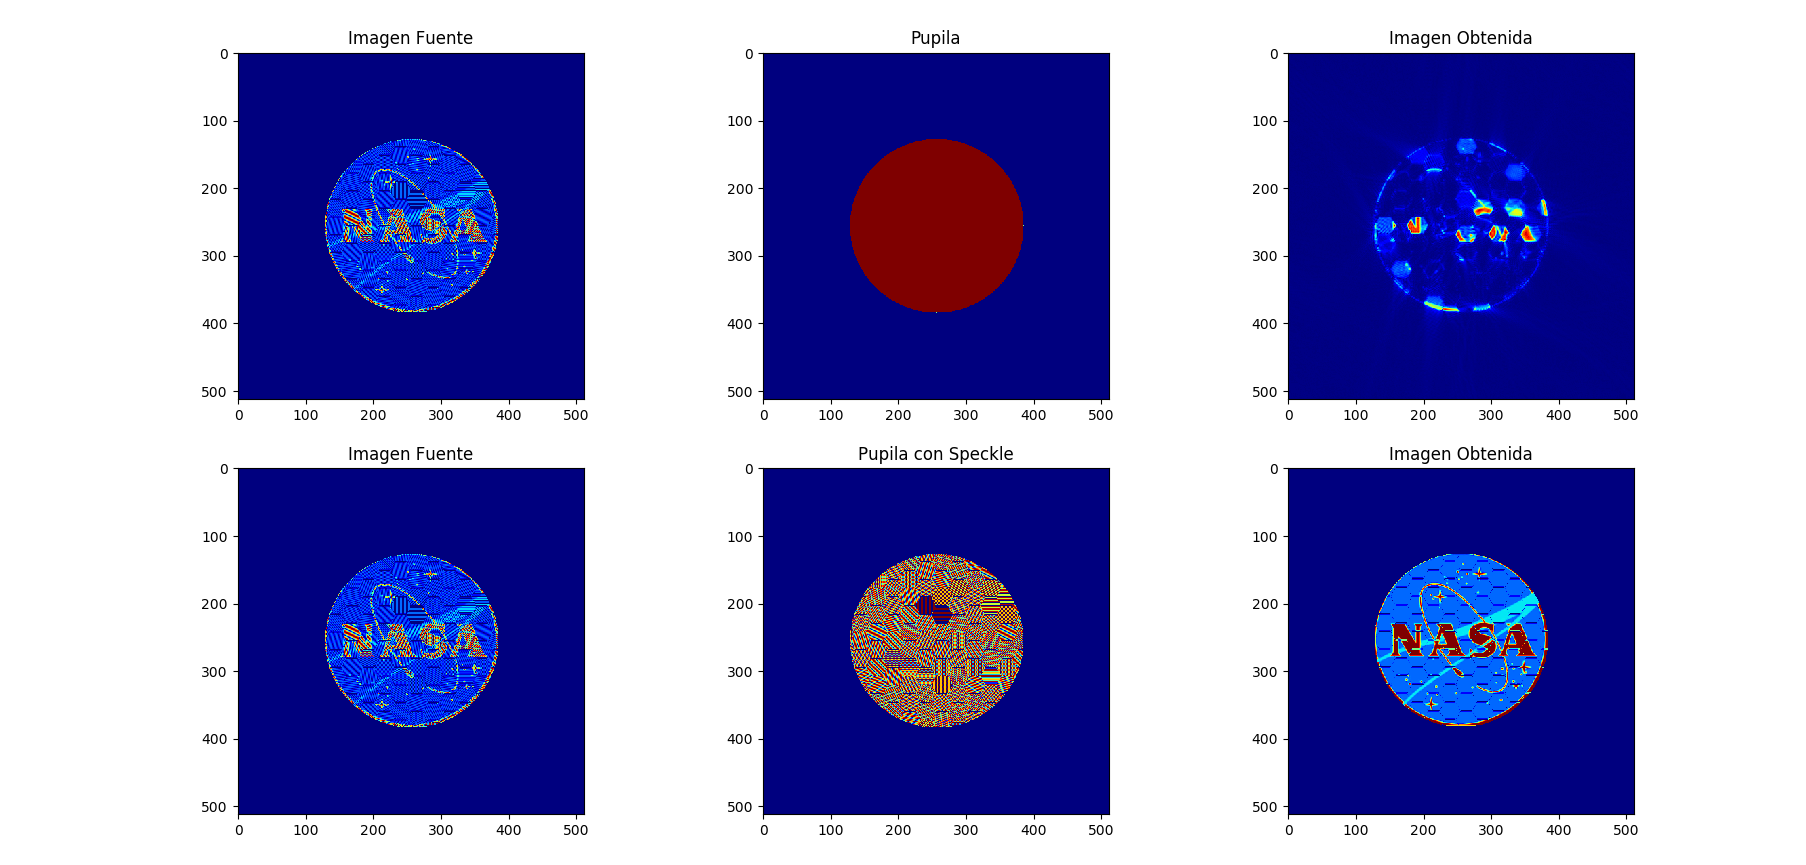
\includegraphics[scale=0.24]{Nasa.png}
						\caption{\label{Img:nasa}Procesamiento de una imagen con fase aleatoria utilizando el método de speckle. La fila de arriba corresponde al procesamiento de imagen sin corrección y la de abajo con corrección mediante pupilas. En la primera columna se muestran las imagenes originales, en la segunda columna el espejo utilizado para su procesamiento y en la tercera columna la imagen obtenida.}
					\end{figure}
				\begin{multicols}{2}
		
		\section{Discusión}

			Se han estudiado las intensidades obtenidas a partir de frentes de onda con fases aleatorias tratando de simular los efectos observados en la atmósfera. 

			En la primera parte se ha estudiado este hecho considerando una fuente puntual, de la cuál se sabe que se ha de obtener la mancha de Airy. En la primera simulación no se ha modificado la fase, obteniendose la mancha de Airy como se puede ver en la figura \ref{Img:airy-normal}. Tras esto se ha decidido utlizar dos espejos formados por pupilas con fases aleatorias. En el primer caso se han utilizado pupilas con un tamaño aproximado al del espejo grande $D \approx r_0$, obteniendo nuevamente la mancha de Airy pero desplazada del centro y con algunas intensidades diferentes como se puede observar en la figura \ref{Img:airy-fase}. Estas pequeñas diferencias con la mancha de Airy de la primera simulación pueden ser debidas a que la forma de la pupila era hexagonal, por lo que una sola pupila no cubría todo el espacio del espejo y aparecían partes de las pupilas continuas en los bordes. Esta pupilas contienen una fase diferente a la de la pupila central, lo que puede originar dichas diferencias. Además, se observa que la pupila central no está perfectamente centrada. 

			El problema de centrar la pupila se podría haber solucionado modificando el código para ello. De igual manera, se podrían haber utilizado pupilas circulares para este caso. Sin embargo, interesaba escribir un código único que permitiese estudiar el fenómeno para diferentes variables. Por ello, de haber utilizado pupilas circulares, en posteriores simulaciones en las que la pupilas son menores, se hubiesen encontrado espacios vacíos.

			En la siguiente simulación se utilizaro  pupilas de tamaño mucho menos al del espejo, siendo 8 veces más pequeñas. Para este caso, se ha podido observar los efectos que produce tener difernecias en la fase de un mismo frente de onda a la hora de obtener su imagen, ya que en la figura \ref{Img:speckle} en la que se muestra el resultado de la simulación, se ha perdido completamente la mancha de Airy.

			Con esta primera parte se ha podido comprobar mediante simulación las aproximaciones de la ecuación \ref{eq:airy}, observando como a medida que $r_0$ disminuye respecto a $D$, se pierde la mancha de Airy.

			Por último, en la última simulación se ha tratado de realizar el procesamiento de imagen de una imagen fuente a la que se le ha aplicado diferentes fases. 

			Se ha podido observar como para este caso, al procesar la imagen sin ninguna correscciónutilizando un espejo sin fase, se pierde completamente la imagen. Esto no es del todo cierto, ya que se pueden intuir partes de la imagen original, ya que la forma de introducirle un desfase a la imagen a sido mediante hexagonos como los de la pupila. Sin embargo, no se puede concluir que se haya obtenido la imagen inicial.

			No obstante, cuando se le ha aplicado un espejo formado por pupilas con una cierta inclinación de tal manera que se aplicase un desfase inverso al de la imagen original, corrigiendo el Speckle, sí se ha podido obtener nuevamente la imagen original exactamente igual.

		\section{Conclusiones}

			Se ha podio estudiar el fenómeno de Speckle pudiendo comprobar mediante una simulación simple las aproximaciones y límites de este fenómeno que se muestran en la ecuación \ref{eq:airy}. Además, se ha podido observar el efecto que este produce a la hora de observar una imagen, volviendo tan dificill las observaciones de estrellas debido a la acción de la atmósfera. Así mismo, se ha simulado las correcciones que se han de realizar a las imagenes para obtener la imagen original.

	\end{multicols}

%----------------------------------------------------------------------------
%     APPENDIX
%----------------------------------------------------------------------------

\newpage

	    \appendix

		    	\section{Obtención del Espejo}
		    		\label{appen:Espejo}

					Para  $(\sqrt{k^2+j^2}=r_{k,j}) < R$:

						\begin{equation}
							Espejo_{k, j} = 1 \cdot e^{i\cdot crv \cdot r_{k,j}} \cdot e^{i\cdot (tip\cdot r_k + tilt \cdot r_j)}
						\end{equation}
						
					Para $(\sqrt{k^2+j^2}=r_{k,j}) = R$:

						\begin{equation}
							Espejo_{k,j} = 0.5 \cdot e^{i\cdot crv \cdot r_{k,j}} \cdot e^{i\cdot (tip\cdot r_k + tilt \cdot r_j)}
							\label{eq:Espejo}
						\end{equation}	

					Siendo $(k, j)$ las coordenadas $(x, y)$ de la matriz, $r_{k, j}$ el radio de esas coordenadas respecto al centro de la matriz, $R$ el radio del espejo, $crv$ la curvatura, $tip$ la inclinación respecto al eje $X$ y $tilt$ la inclinación respecto al eje $Y$.
	    		
%----------------------------------------------------------------------------
%     BIBLIOGRAPHY
%----------------------------------------------------------------------------

	\bibliographystyle{unsrt}
	\bibliography{biblio}

\end{document}


%----------------------------------------------------------------------------
%            TEMPLATES
%----------------------------------------------------------------------------

%----------------------------------------------------------------------------
%            how to insert an image
%----------------------------------------------------------------------------

%	\begin{figure}[H]
%		\centering
%		\includegraphics[scale= ]{nombre de la imagen.jpg}
%		\caption{\label{Img:widgets}el pie de pagina que le quieras 	poner a la imagen}
%	\end{figure}
 
%----------------------------------------------------------------------------
%            how to insert a table
%----------------------------------------------------------------------------

%	\begin{table}[H]
%		\centering
%		\begin{tabular}{|c|c|c|c|}
%			\hline
%			\centering
%				Altura(h) & Distancia (d) & Elaboracion (e) & Longitud (l) \\
%				($\pm0.5$ mm) & ($\pm0.5$ mm) & ($\pm0.5$ mm) & ($\pm0.5$ mm) \\ \hline
%				 &  &  &  \\ \hline
%				 &  &  &  \\ \hline
%				 &  &  &  \\ \hline
%				 &  &  &  \\ \hline
%				 &  &  &  \\ \hline
%		         &  &  &  \\ \hline
%		\end{tabular}
%		\caption{\label{Tab:widgets}pie de pagina que le quieras poner}
%	\end{table}

%----------------------------------------------------------------------------
%             How to remove the label in equactions
%----------------------------------------------------------------------------

%	\begin{equation*}
%		
%	\end{equation*}

%----------------------------------------------------------------------------
%              How to set bibliography
%----------------------------------------------------------------------------

%\bibliographystyle{unsrt}
%\bibliography{biblio}
%
%Then you have to set a .bib document such as the next template
%
%	@book{nickname,
%	author = {},
%	title = {},
%	edition = {},
%	year = {},
%	volume = {},
%	ISBN = {}
%	}
%
%	@ARTICLE{nickname,
%	author = {},
%	title = {},
%	year = {},
%	volume = {},
%	}


%----------------------------------------------------------------------------
%              END
%----------------------------------------------------------------------------
